\documentclass[a4paper]{article}
\usepackage{amsfonts}
\usepackage{amsmath}
\addtolength{\hoffset}{-2.25cm}
\addtolength{\textwidth}{4.5cm}
\addtolength{\voffset}{-3.25cm}
\addtolength{\textheight}{5cm}
\setlength{\parindent}{15pt}

\usepackage[unicode=true, colorlinks=false, hidelinks]{hyperref}
\usepackage[utf8]{inputenc}
\usepackage[english, russian]{babel}
\usepackage{mathtext}
\usepackage[T2A, TS1]{fontenc}
\usepackage{microtype} % Slightly tweak font spacing for aesthetics
\usepackage{amsthm, amssymb, amsmath, amsfonts, nccmath}
\usepackage{nicefrac}
\usepackage{epstopdf}
\usepackage[export]{adjustbox}
\usepackage{float} % Improved interface for floating objects
\usepackage{graphicx, multicol} % Enhanced support for graphics
\usepackage{pdfrender,xcolor}
\usepackage{breqn}
\usepackage{mathtools}
\usepackage{titling}
\usepackage{bm}
\usepackage{centernot}
\usepackage[cal=boondoxo,calscaled=.96]{mathalpha}
\usepackage{marvosym, wasysym} % More symbols
\usepackage{rotating} % Rotation tools
\usepackage{censor} % Facilities for controlling restricted text

\usepackage{fancyhdr}
\pagestyle{fancy}
\fancyhead{}\renewcommand{\headrulewidth}{0pt}
\fancyfoot[L]{}
\fancyhead{}
\fancyfoot{}
\fancyfoot[R]{\thepage}
\begin{document}
    \begin{titlepage}
   \begin{center}
       \vspace*{3cm}
       \large{САНКТ-ПЕТЕРБУРГСКИЙ ПОЛИТЕХНИЧЕСКИЙ УНИВЕРСИТЕТ}
       \vspace{0.4 cm}

       \large\textbf{Институт прикладной математики и механики}
       \vspace{0.4 cm}

       \large{Высшая школа прикладной математики и вычислительной физики}

       \vspace{3 cm}
       \normalsize\textbf{Отчет\\ по лабораторной работе №7\\ по дисциплине\\
«Математическая статистика»}
       \vfill
       \begin{flushright}
            \normalsize{Выполнил студент:\\
            Антонов Алексей\\
            группа: 3630102/80201}
            \vskip\medskipamount
            \normalsize{Проверил:

            к.ф.-м.н., доцент\\
            Баженов Александр Николаевич
            }
       \end{flushright}

       \vspace{0.8cm}


       \normalsize{Санкт-Петербург\\2021 г.}

   \end{center}
\end{titlepage}
    \tableofcontents
    \newpage
	\listoffigures
    \newpage
\section {Постановка задачи}
\noindent Сгенерировать выборки размером 20, 60 и 100 элементов. Построить на них эмпирические функции распределения и ядерные оценки плотности распределения на отрезке $[-4;\,4]$ для непрерывных распределений и на отрезке $[6;\,14]$ для распределения Пуассона.

\section {Теория}
\subsection{Эмпирическая функция распределения}
\subsubsection{Статистический ряд}
\noindent Статистическим рядом назовем совокупность, состоящую из последовательности $\displaystyle\{z_i\}_{i=1}^k$ попарно различных элементов выборки, расположенных по возрастанию, и последовательности $\displaystyle\{n_i\}_{i=1}^k$ частот, с которыми эти элементы содержатся в выборке.
\subsubsection{Эмпирическая функция распределения}
\noindent Эмпирическая функция распределения (э. ф. р.) - относительная частота события $X < x$, полученная по данной выборке:
\begin{equation}
    F_n^*(x)=P^*(X<x).
\end{equation}
\subsubsection{Нахождение э. ф. р.}
\begin{equation}
    F^*(x)=\frac{1}{n}\sum_{z_i<x}n_i.
\end{equation}
$F^*(x)-$ функция распределения дискретной случайной величины $X^*$, заданной таблицей распределения
\begin{table}[H]
    \centering
    \begin{tabular}{|c|c|c|c|c|}
        \hline
         $X^*$&$z_1$&$z_2$&...&$z_k$\\
         \hline
         $P$&$n_1/n$&$n_2/n$&...&$n_k/n$\\
         \hline
    \end{tabular}
    \caption{Таблица распределения}
    \label{tab:my_label}
\end{table}
\noindent Эмпирическая функция распределения является оценкой, т. е. приближённым значением, генеральной функции распределения
\begin{equation}
    F_n^*(x)\approx F_X(x).
\end{equation}
\subsection{Оценки плотности вероятности}
\subsubsection{Определение}
\noindent Оценкой плотности вероятности $f(x)$ называется функция $\widehat{f}(x)$, построенная на основе выборки, приближённо равная $f(x)$
\begin{equation}
    \widehat{f}(x)\approx f(x).
\end{equation}
\subsubsection{Ядерные оценки}
\noindent Представим оценку в виде суммы с числом слагаемых, равным объёму выборки:
\begin{equation}
    \widehat{f}_n(x)=\frac{1}{n h_n}\sum_{i=1}^n K\left(\frac{x-x_i}{h_n}\right).
\end{equation}
$K(u)$ - ядро, т. е. непрерывная функция, являющаяся плотностью вероятности, $x_1,...,x_n$ $-$ элементы выборки, а $\{h_n\}_{n\in\mathbb{N}}$ - последовательность элементов из $\mathbb{R}_+$ такая, что
\begin{equation}
    h_n\xrightarrow[n\to\infty]{}0;\;\;\;n h_n\xrightarrow[n\to\infty]{}\infty.
\end{equation}
Такие оценки называются непрерывными ядерными.\\\\
Гауссово ядро:
\begin{equation}
    K(u)=\frac{1}{\sqrt{2\pi}}e^{-\frac{u^2}{2}}.
\end{equation}
Правило Сильвермана:
\begin{equation}
    h_n=\left(\frac{4\hat{\sigma}^5}{3n}\right)^{1/5}\approx1.06\hat{\sigma}n^{-1/5},
\end{equation}
где $\hat{\sigma}$ - выборочное стандартное отклонение.

\section{Программная реализация}
Лабораторная работа выполнена на языке Python в среде PyCharm с использованием следующих библиотек:
\begin{enumerate}
    \item numpy
    \item scipy
    \item matplotlib
\end{enumerate}


\section {Результаты}
\subsection{Эмпирическая функция распределения}
	\begin{figure}[H]
	\centering
	\centering
	{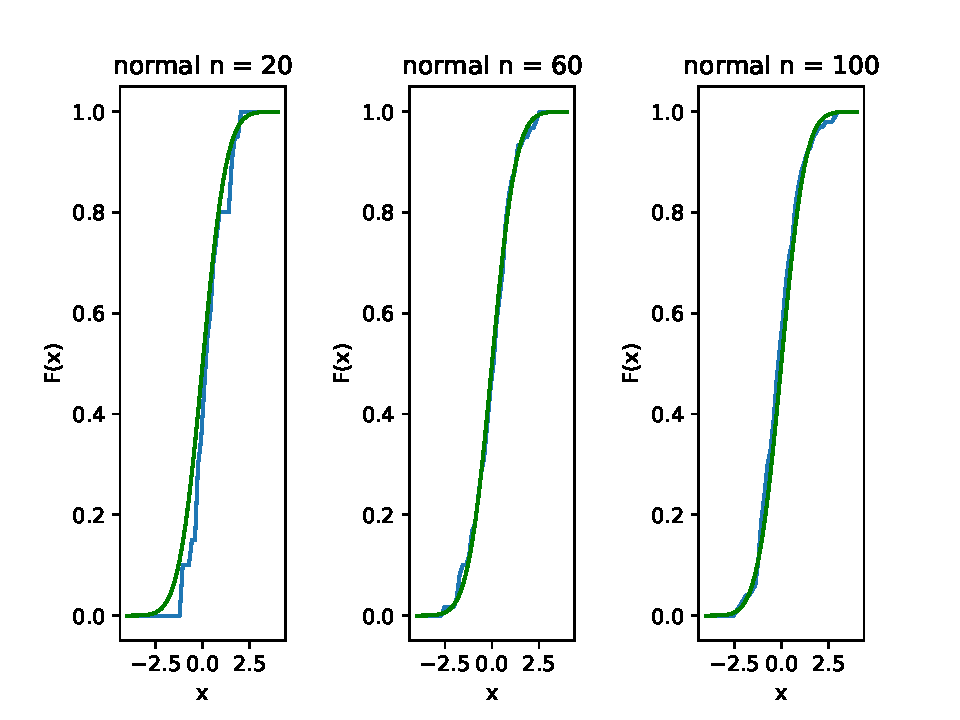
\includegraphics[scale=0.5]{src/emperical_fun_normal}}
		\caption{Нормальное распределение}
		\label{fig:normal}
	\end{figure}

\begin{figure}[H]
	\centering
	{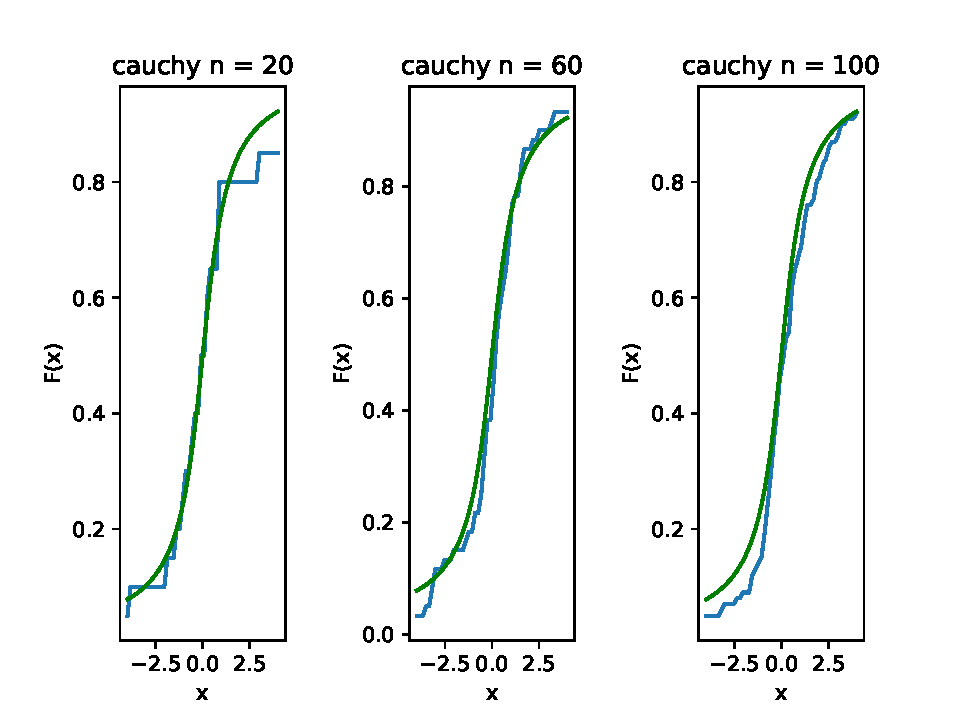
\includegraphics[scale=0.5]{src/emperical_fun_cauchy}}
		\caption{Распределение Коши}
		\label{fig:cauchy}
	\end{figure}

\begin{figure}[H]
	\centering
	{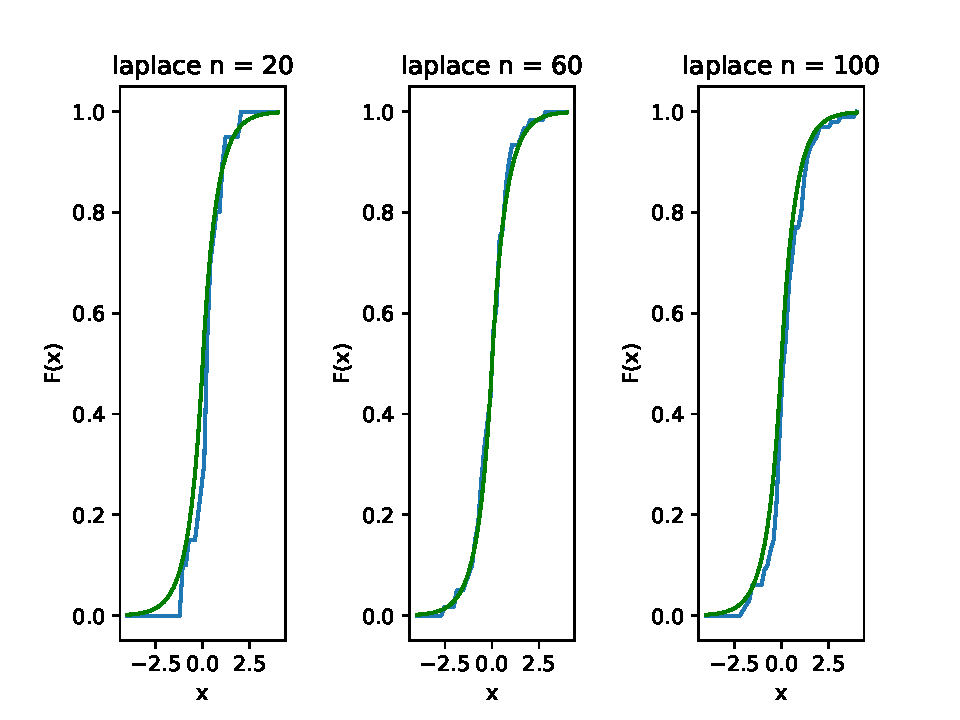
\includegraphics[scale=0.5]{src/emperical_fun_laplace}}
		\caption{Распределение Лапласа}
		\label{fig:laplace}
	\end{figure}

\begin{figure}[H]
	\centering
	{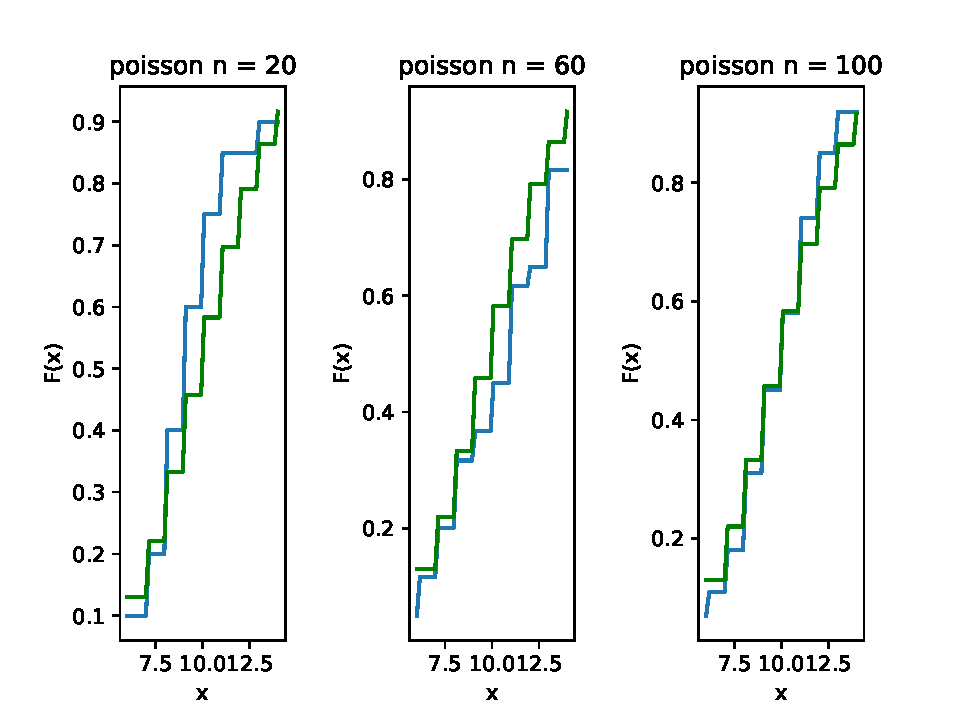
\includegraphics[scale=0.5]{src/emperical_fun_poisson}}
		\caption{Распределение Пуассона}
		\label{fig:posson}
	\end{figure}

\begin{figure}[H]
	\centering
	{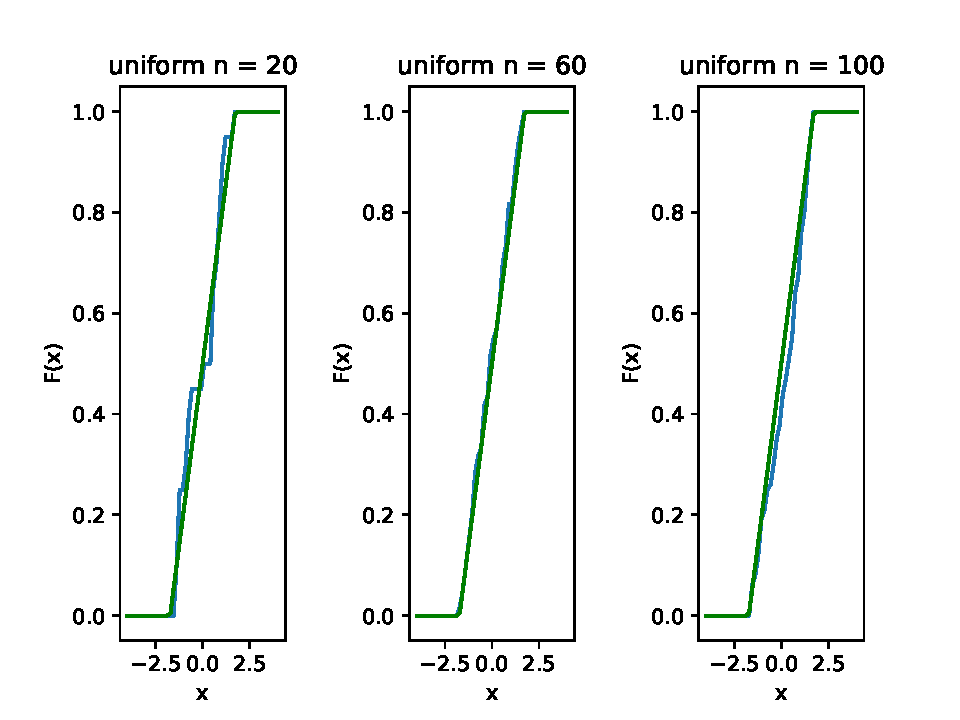
\includegraphics[scale=0.5]{src/emperical_fun_uniform}}
		\caption{Равномерное распределение}
		\label{fig:uniform}
	\end{figure}

\subsection{Ядерные оценки плотности распределения}
\begin{figure}[H]
	\centering
	{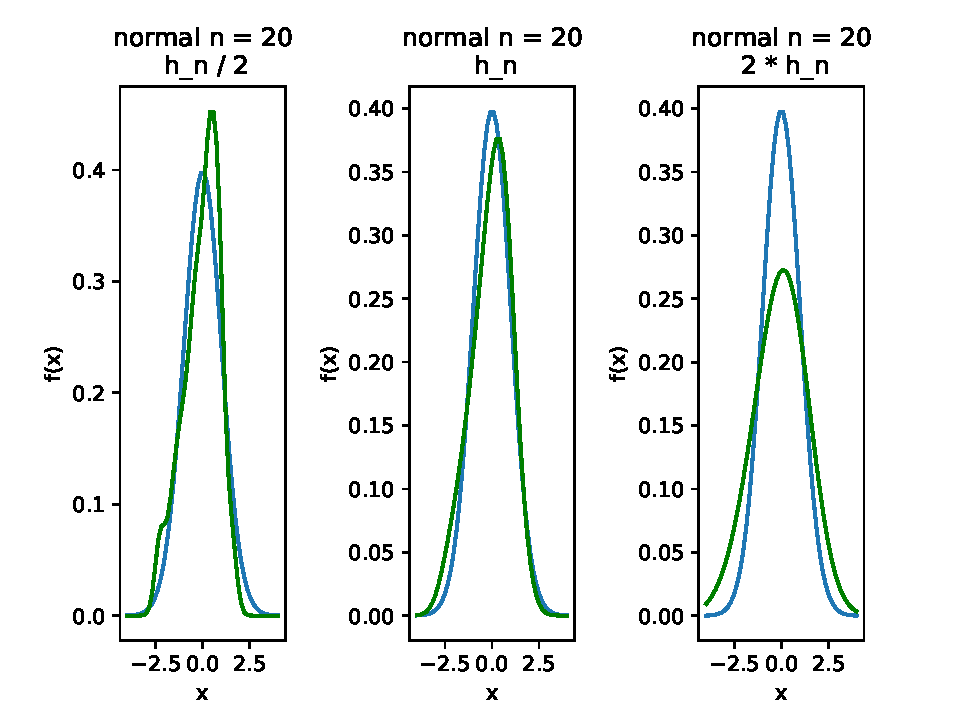
\includegraphics[scale=0.5]{src/kde_20_normal}}
		\caption{Нормальное распределение, $n=20$}
		\label{fig:kde_normal_20}
	\end{figure}

\begin{figure}[H]
	\centering
	{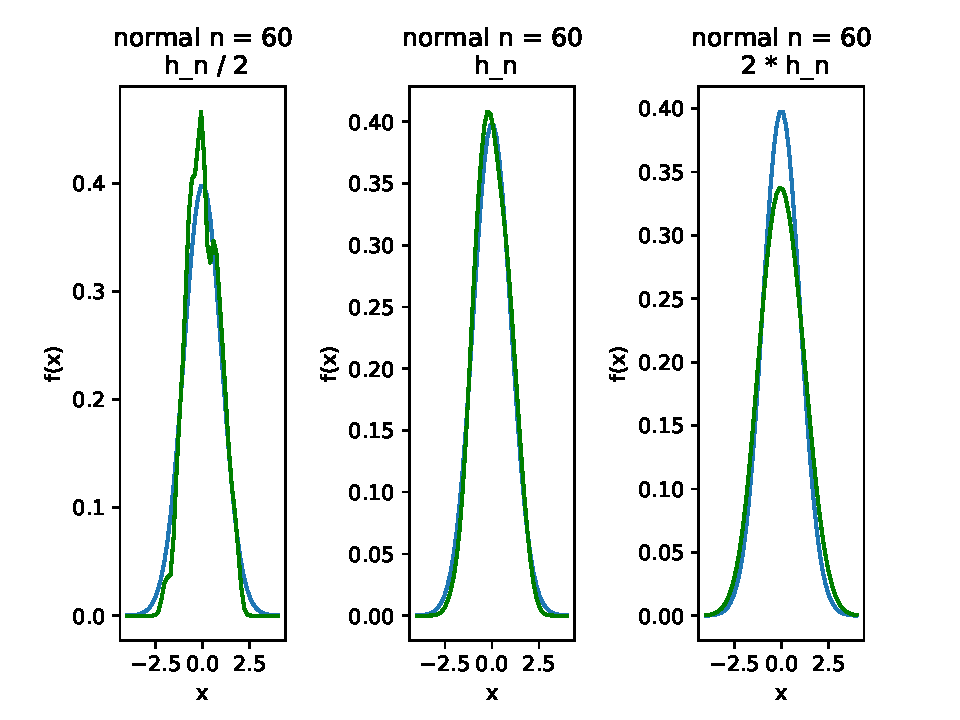
\includegraphics[scale=0.5]{src/kde_60_normal}}
		\caption{Нормальное распределение, $n=60$}
		\label{fig:kde_normal_60}
	\end{figure}

\begin{figure}[H]
	\centering
	{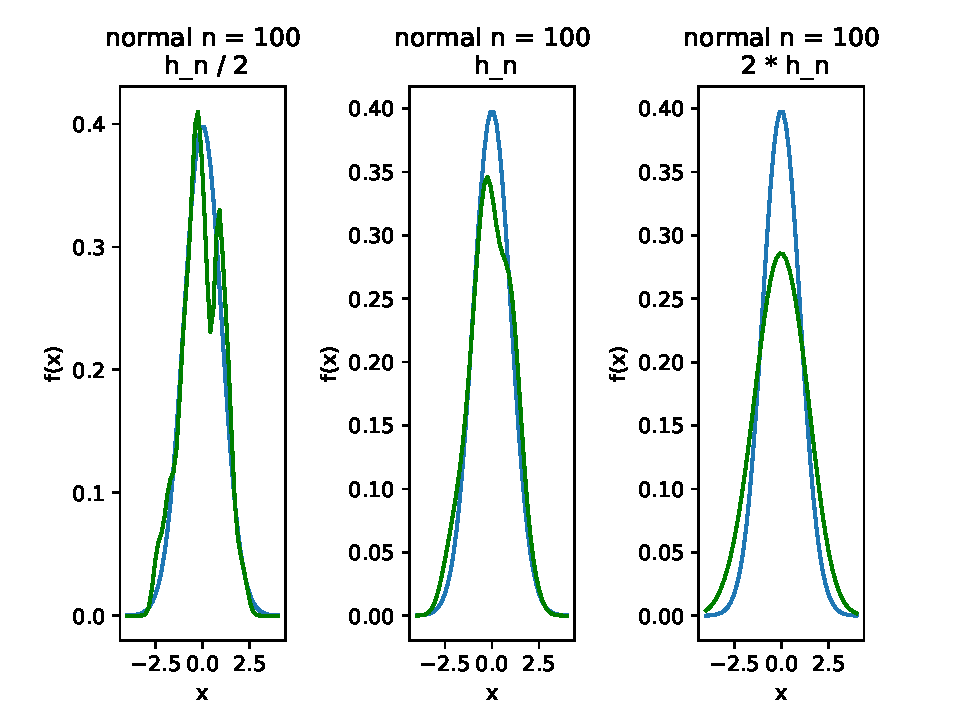
\includegraphics[scale=0.5]{src/kde_100_normal}}
		\caption{Нормальное распределение, $n=100$}
		\label{fig:kde_normal_100}
	\end{figure}

\begin{figure}[H]
	\centering
	{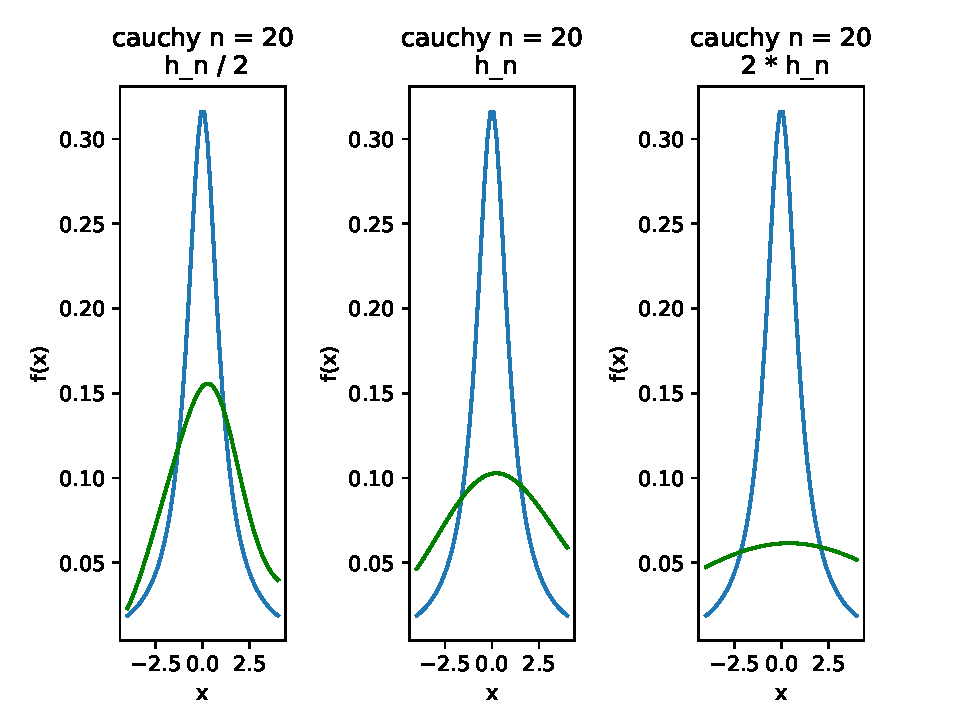
\includegraphics[scale=0.5]{src/kde_20_cauchy}}
		\caption{Распределение Коши, $n=20$}
		\label{fig:kde_cauchy_20}
	\end{figure}

\begin{figure}[H]
	\centering
	{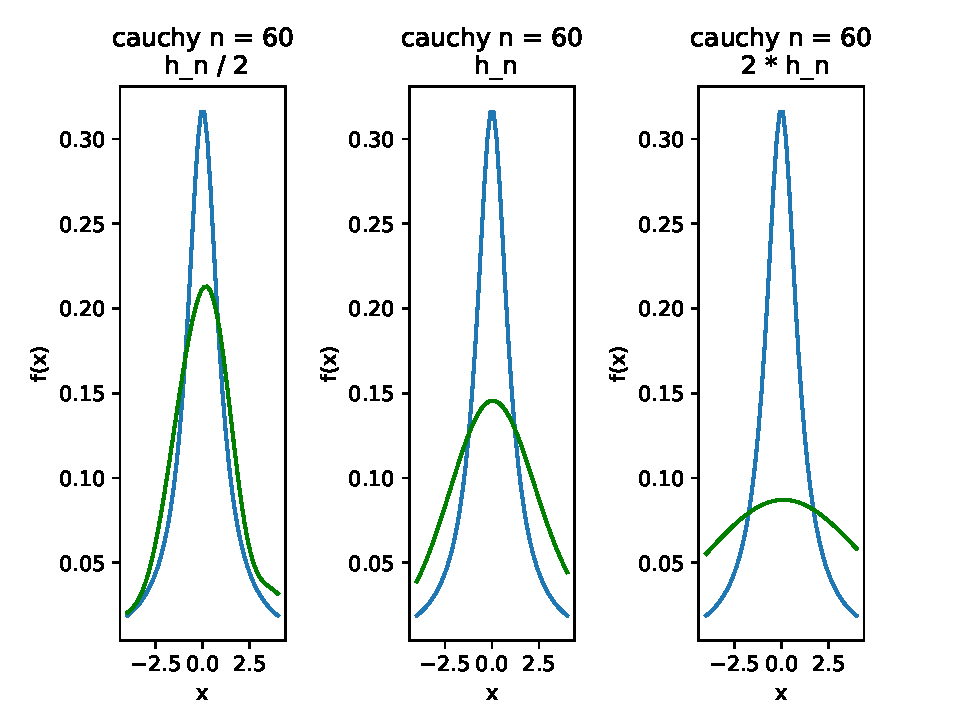
\includegraphics[scale=0.5]{src/kde_60_cauchy}}
		\caption{Распределение Коши, $n=60$}
		\label{fig:kde_cauchy_60}
	\end{figure}

\begin{figure}[H]
	\centering
	{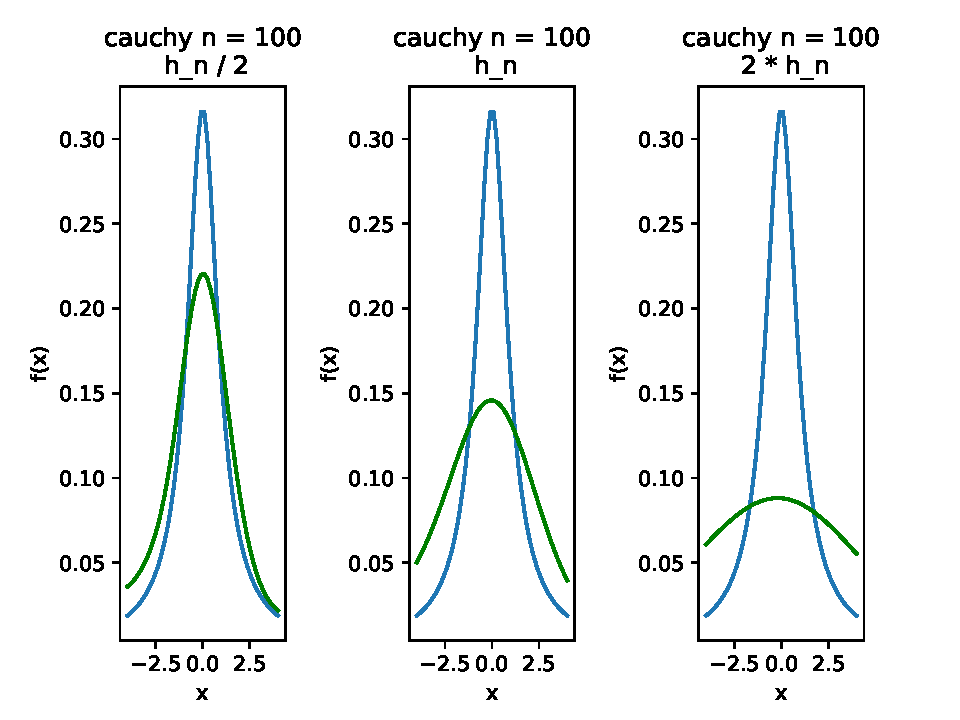
\includegraphics[scale=0.5]{src/kde_100_cauchy}}
		\caption{Hаспределение Коши, $n=100$}
		\label{fig:kde_cauchy_100}
	\end{figure}

\begin{figure}[H]
	\centering
	{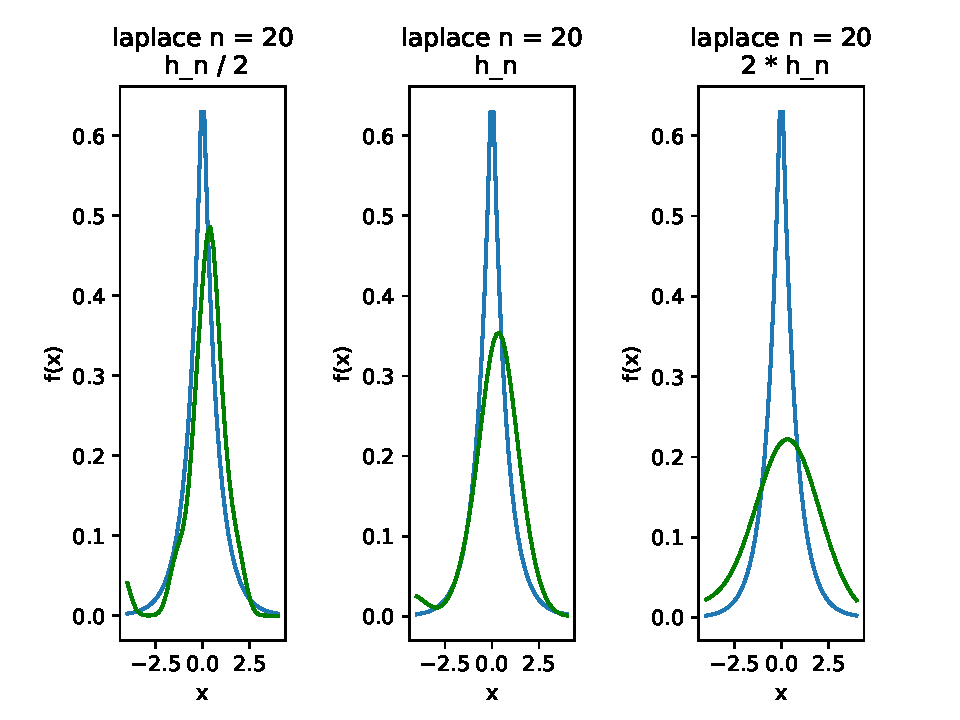
\includegraphics[scale=0.5]{src/kde_20_laplace}}
		\caption{Распределение Лапласа, $n=20$}
		\label{fig:kde_laplace_20}
	\end{figure}

\begin{figure}[H]
	\centering
	{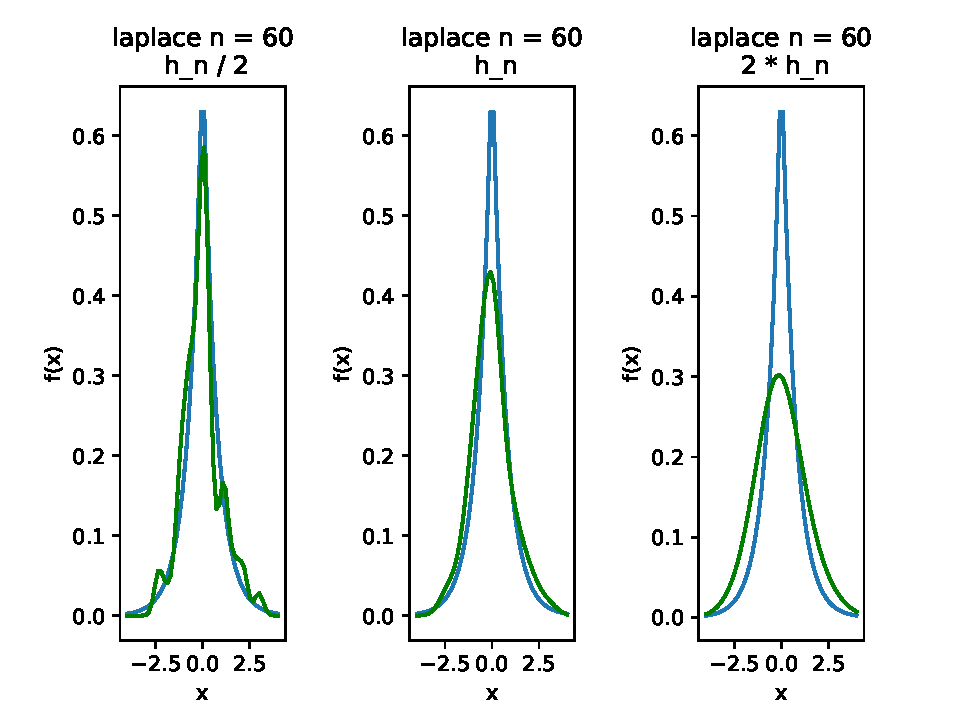
\includegraphics[scale=0.5]{src/kde_60_laplace}}
		\caption{Распределение Лапласа, $n=60$}
		\label{fig:kde_laplace_60}
	\end{figure}

\begin{figure}[H]
	\centering
	{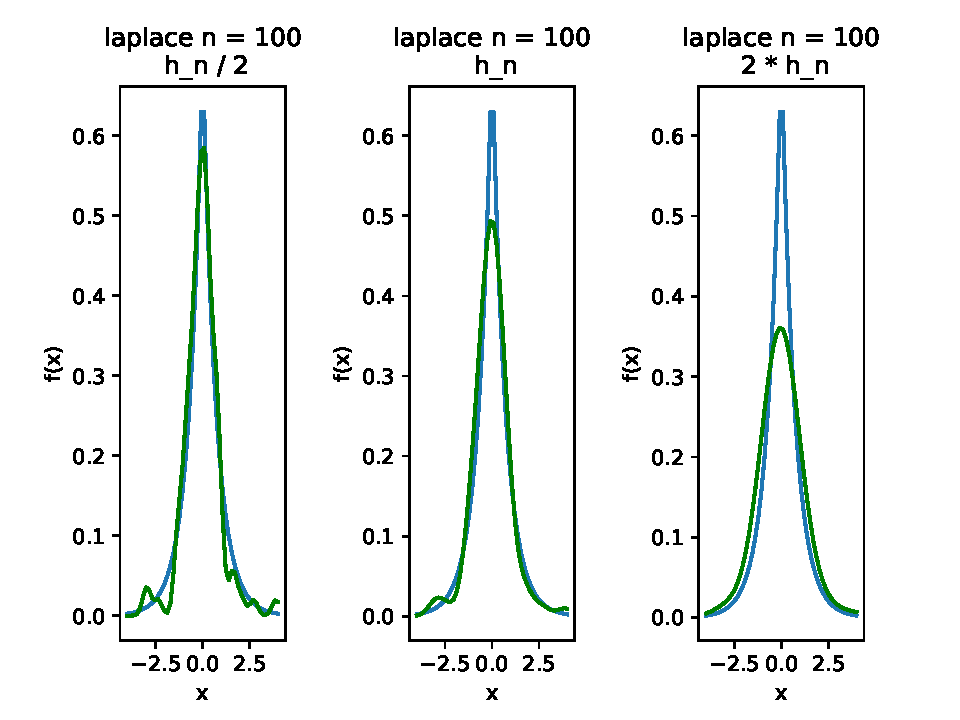
\includegraphics[scale=0.5]{src/kde_100_laplace}}
		\caption{Распределение Лапласа, $n=100$}
		\label{fig:kde_laplace_100}
	\end{figure}

\begin{figure}[H]
	\centering
	{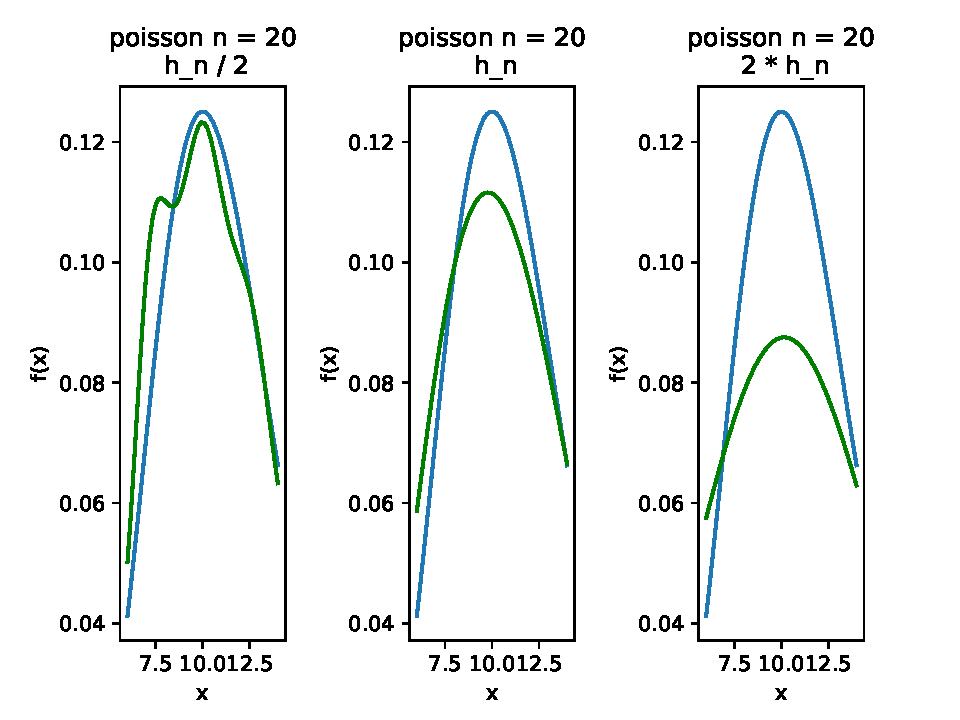
\includegraphics[scale=0.5]{src/kde_20_poisson}}
		\caption{Распределение Пуассона, $n=20$}
		\label{fig:kde_poisson_20}
	\end{figure}

\begin{figure}[H]
	\centering
	{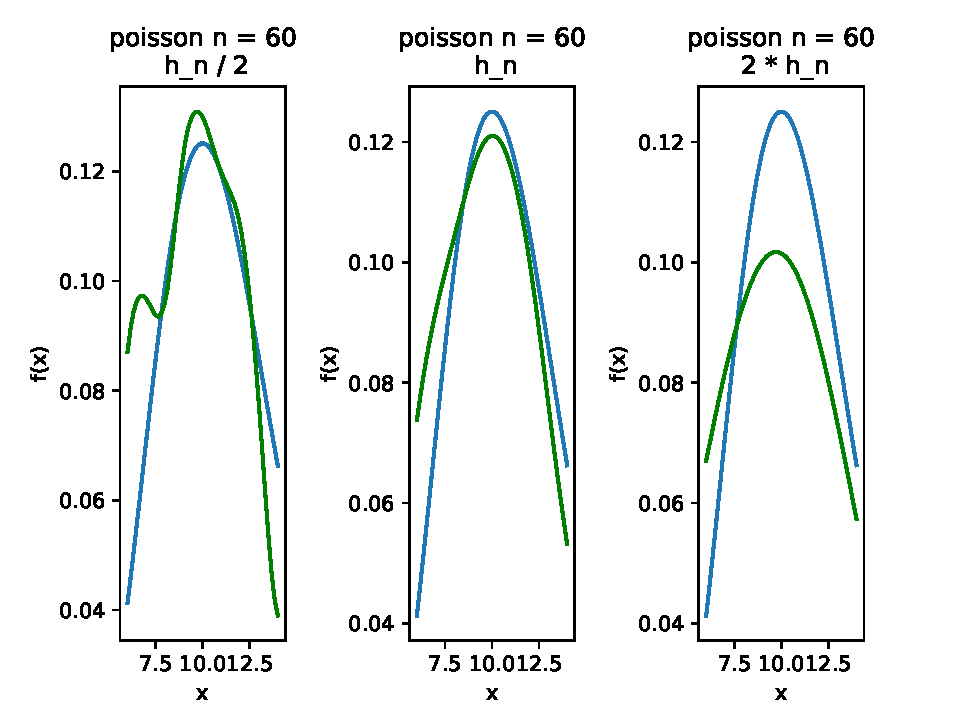
\includegraphics[scale=0.5]{src/kde_60_poisson}}
		\caption{Распределение Пуассона, $n=60$}
		\label{fig:kde_poisson_60}
	\end{figure}

\begin{figure}[H]
	\centering
	{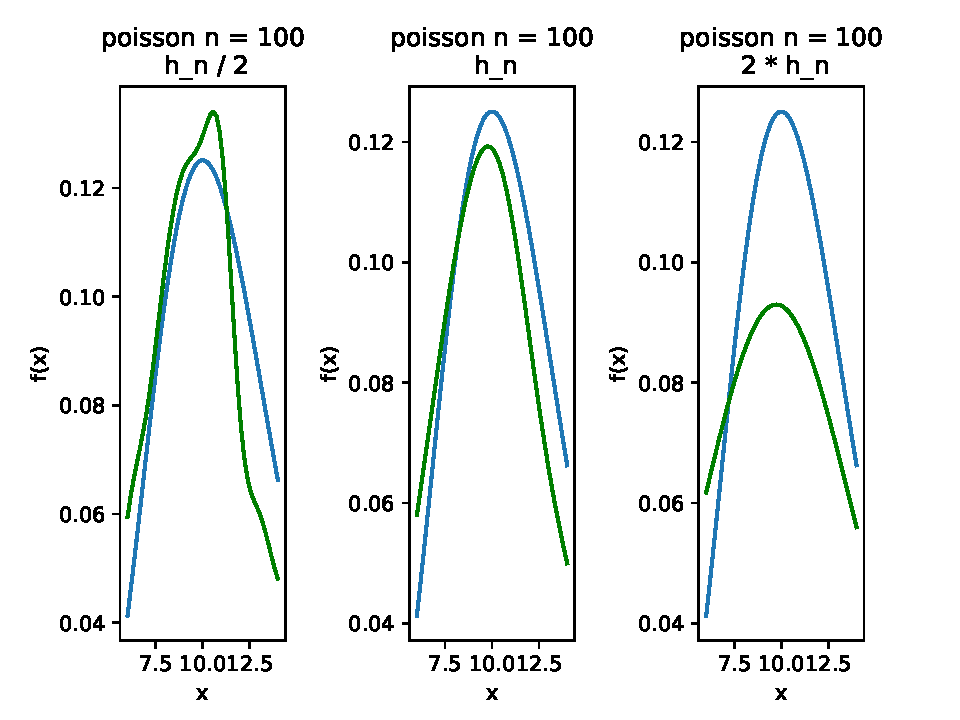
\includegraphics[scale=0.5]{src/kde_100_poisson}}
		\caption{Распределение Пуассона, $n=100$}
		\label{fig:kde_poisson_100}
	\end{figure}

\begin{figure}[H]
	\centering
	{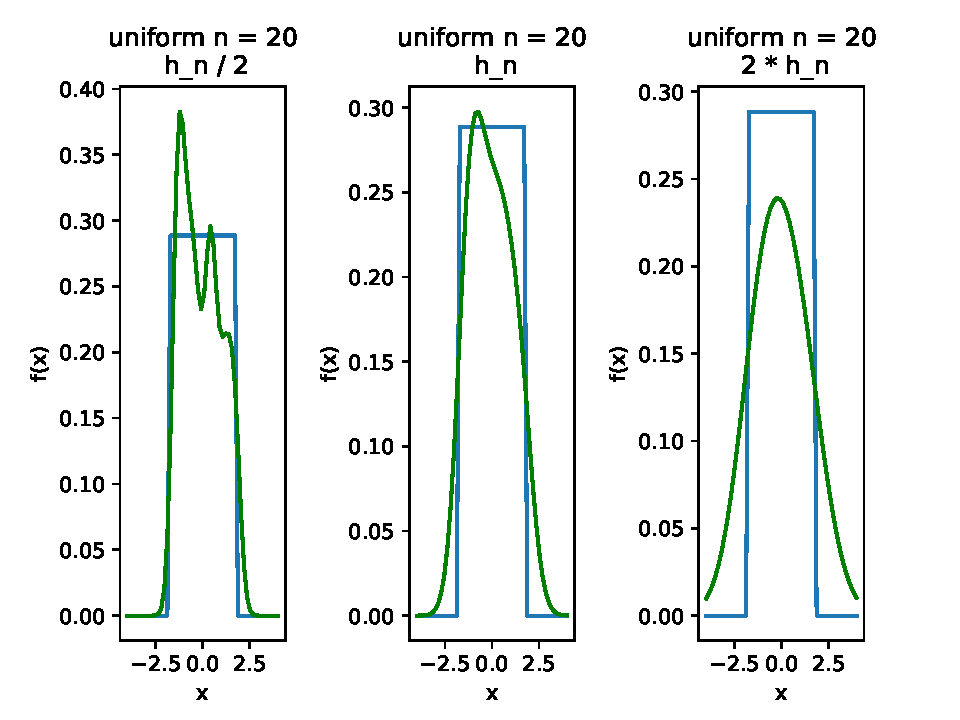
\includegraphics[scale=0.5]{src/kde_20_uniform}}
		\caption{Равномерное распределение, $n=20$}
		\label{fig:kde_uniform_20}
	\end{figure}

\begin{figure}[H]
	\centering
	{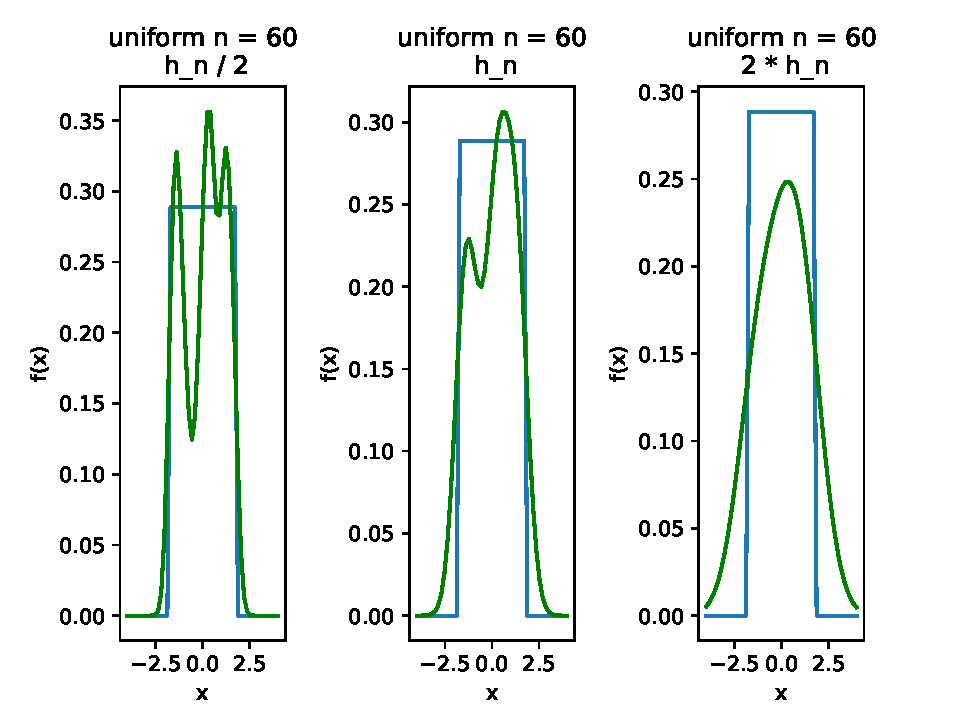
\includegraphics[scale=0.5]{src/kde_60_uniform}}
		\caption{Равномерное распределение, $n=60$}
		\label{fig:kde_uniform_60}
	\end{figure}

\begin{figure}[H]
	\centering
	{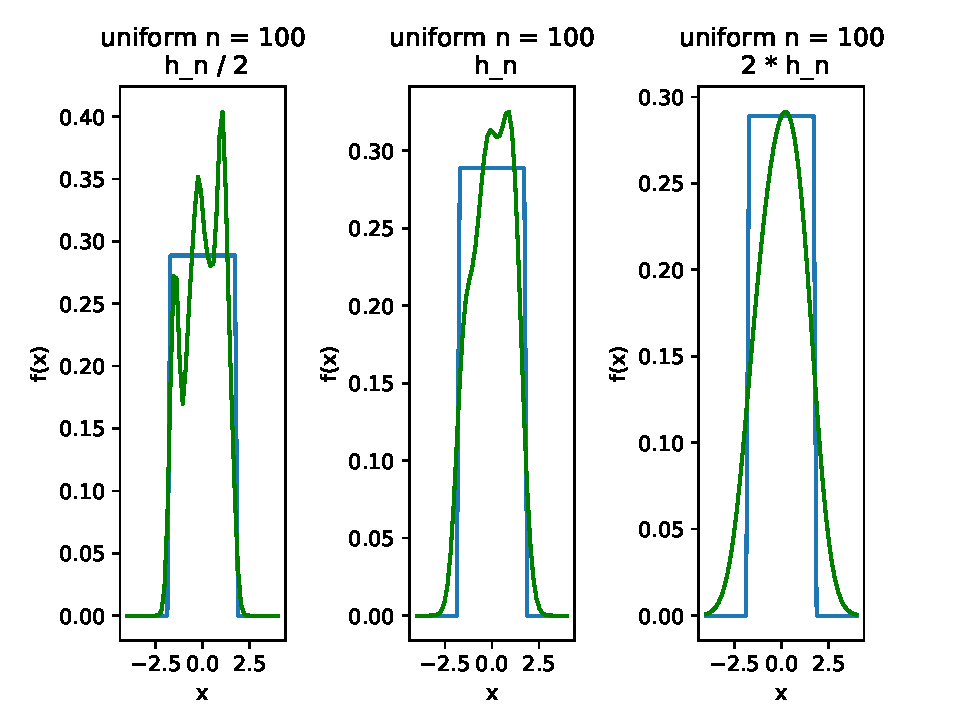
\includegraphics[scale=0.5]{src/kde_100_uniform}}
		\caption{Равномерное распределение, $n=100$}
		\label{fig:kde_uniform_100}
	\end{figure}
\section{Обсуждение}
На представленных графиках видно, что эмпирическая функция распределения тем лучше приближает функцию распределения заказа, чем больший объем выборки мы берём. Наибольшие отклонения наблюдаются для распределения Пуассона и равномерного распределения.


По иллюстрациям, относящимся к ядерным оценкам плотности вероятности можно увидеть, что снова качество приближения увеличивается с увеличением размеров выборки. При этом выбор оптимального параметра h отличается для разных распределений. Например, для распределения Лапласа лучшие результаты даёт $h_n=0.5$

Чем больше числовой коэффициент при параметре сглаживания $h_n$, тем менньшее количество раз происходит чередование знака производной аппроксимирующей функции на рассматриваемом промежуткем. При выборе коэффициента равного 2 мы приходим к цнимодальной функции и полученные приближения перестают описывать особенности распределения, так что становится невозможно сказать что-то о законе распредления случайной величины.



\section{Приложение}

С кодом работы и отчета можно ознакомиться по ссылке:\;\url{https://github.com/sqrtyyy/MathStat/tree/master/lab_4}
\end{document}